% ----------------------------------------------
% ----------------------------------------------
% \subsection{Traditional adversarial label introduces label noise implicitly} 
% \section{Label noise implicitly exists in the adversarially augmented training set}
\section{Label noise implicitly exists in adversarial training}
\label{sect:reason}
% \label{sect:implicit-label-noise}
    
    In this section, we demonstrate the implicit existence of label noise in the adversarially augmented training set. We first consider a simple case where the adversarial perturbation is generated based on an ideal classifier that predicts the true label distribution. Under such a case we prove that the label noise in the adversarially augmented training set is lower-bounded. We then show that in realistic cases an adversarially trained classifier can approximate the true label distribution with high probability. Therefore, additional error terms will be required to lower bound the label noise.
    % Although traditional adversarial label is unlikely to directly produce label flipping noise, 
    % i.e., ``$\argmax_j ~p(y_\delta=j|x + \delta) = \argmax_j ~p(y=j|x)$'', 
    % we show that it can produce label noise implicitly. 
    All proofs for the remainder of this paper are provided in the appendix.
    
    % \chengyu{The general idea is after adversarial perturbation, the true label distribution is distorted, while the assigned label distribution doesn't change, creating a distribution mismatch between the true label distribution and the assigned label distribution.}

    % It has been widely observed that adversarial examples transfer between different classifiers even with distinct architectures~\citep{Papernot2017PracticalBA}. Meanwhile, 

    %% Mentioned in introduction
    % An adversarial example often contains salient characteristics of classes other than the original label from human perspective~\citep{Tsipras2019RobustnessMB,Ilyas2019AdversarialEA}. This implies that the true label distribution of an adversarial example is likely to be different from its clean counterpart. %  which means $P(Y^*_\delta | x_\delta) \ne P(Y^* | x)$. 

    % Note this will not conflict with $y^*_\delta = y^*$ as discussed in Section~\ref{sect:label-flipping-noise}, since the latter only implies $\argmax_j ~P(Y^*_\delta=j|x_\delta) = \argmax_j ~P(Y^*=j|x)$.
    % Therefore, the adversarial perturbation is likely to distort the ground-truth label distribution of an example, which means $p( y_{\delta} | x + \delta) \ne p( y | x)$. 


       
    \subsection{When adversarial perturbation is generated by the true probabilistic classifier}
    \label{sect:reason-true}
    % \jingbo{shall we say true or oracle?}
    % \chengyu{It is adversarial perturbation to optimal label function, not optimal adversarial perturbation. Because we eventually use FGSM and it won't necessarily optimally increase the loss.}
    We first consider an ideal case where the adversarial perturbation is generated by the true probabilistic classifier $f(x):= P(Y|x)$, namely the classifier producing the true label distribution on any input $x$.
    % Adversarial perturbation generated by the true model will definitely shift the true label distribution.
        
    % Show label noise exists with optimal adversarial perturbation, but removing local convexity assumption, just use the intermediate value theorem. 
    
    % \chengyu{Later, in ``factors'' section, introduce assumption of the connection between gradient and data quality, and thus prove the factors of data quality. (Note the difference between $\nabla_x f(z)_y$ and $\nabla_x f(x)_y$ can be bounded with local Lipschitz assumption. Thus should be okay to use $\nabla_x f(x)_y$ as a data quality indicator.)}

    
    % --------------------------------------------------
    % --------------------------------------------------
    % -----------------------------------------------------
    \smallsection{The true label distribution is distorted by adversarial perturbation}
    % \chengyu{We think after adversarial perturbation the true label distribution will be different based on analysis of optimal perturbation. We quantify the magnitude of such distribution shift.}
    We quantify the mismatch between two probability distributions using the \emph{total variation (TV) distance}.
    \begin{definition}[TV distance]
    \label{definition:total-variation-distance}
    % Let $J$ be a subset of the label sample space $\mathcal{Y}$.
    Let $\mathcal{A}$ be a collection of the subsets of the label sample space $\mathcal{Y}$. The TV distance between two probability distributions $P(Y)$ and $P(Y')$ can be defined as $
    %  \small
       \|P(Y) - P(Y')\|_{\text{TV}} = \sup_{J\in \mathcal{A}} \left| P(Y\in J) - P(Y'\in J)\right| 
    %   \normalsize
      $.
    \end{definition}
    
    We now show that adversarial perturbation generated by the true probabilistic classifier can induce a mismatch between the true label distributions of clean inputs and their adversarial examples.
    For simplicity we consider adversarial perturbation based on FGSM and cross-entropy loss, namely $x' = x -\varepsilon \|\nabla~f(x)_y\|^{-1} \nabla~f(x)_y$.
    The distribution mismatch induced by such adversarial perturbation can be lower bounded.
    % With mild assumptions on the true label distribution, we show that such distribution mismatch is lower bounded.
    \begin{lemma}
    % [Distribution mismatch under adversarial perturbation]
    \label{theorem:distribution-mismatch-true-model}
    % Assume the true label distribution $p_Y$ is locally convex around $x$,
    % Let $f(x)_y = P(Y=y|x)$ be the probability mass at class $y$ of the true label distribution of $x$.
    % Assume $f(x)_y$ is twice continuously differentiable with Hessian bounded above around $x$. % i.e. $\|\nabla^2_x P(Y=j|x)\|_2 \le M$,
    % Assume the true label distribution $P(Y=y|x)$ is locally quasiconvex around $x$,
    Assume $f(x)_y$ is $L$-locally Lipschitz around $x$ with bounded Hessian. Let $\sigma_m = \inf_{z \in \mathcal{B}_\varepsilon(x)} \sigma_{\min} (\nabla^2 f(z)_y) > 0$ and $\sigma_M = \sup_{z \in \mathcal{B}_\varepsilon(x)} \sigma_{\max} (\nabla^2 f(z)_y) > 0$.
    Here $\sigma_{\min}$ and $\sigma_{\max}$ denote the minimum and maximum eigenvalues of the Hessian, respectively.
    We then have
    \begin{equation}
        % % P(Y'\ne Y | x) \ge
        % % \frac{1}{2}[\epsilon\|\nabla_x f(z)_y\|_\infty]
        \|P(Y|x) - P(Y'|x')\|_{\text{TV}} \ge
        % \frac{\varepsilon}{2}  \|\nabla_x f(x)_y\|_2 - \frac{\varepsilon^2}{4} M
        % \|p_Y - p_{Y'}\|_{\text{TV}} > 0.
        \frac{\varepsilon}{2} (1 - f(x)_y) \frac{\sigma_m}{L}  - \frac{\varepsilon^2}{4} \sigma_M,
    \end{equation}
    \end{lemma}

    One can find that the right-hand side is positive as long as the upper bound of the Hessian norm is not too large, which is reasonable as previous works have shown that small hessian norm is critical to both standard~\citep{Keskar2017OnLT} and robust generalization~\citep{MoosaviDezfooli2019RobustnessVC}.
    % because it is second-order term, so don't have to be too small.


    
    % -------------------------------------------------------
    % -------------------------------------------------------
    \smallsection{Assigned label distribution is unchanged} Despite the fact that the true label distribution is distorted by adversarial perturbation, we note that the assigned label distribution of adversarial examples is still the same as their clean counterparts.
    \begin{remark} % [Label construction in adversarial training]
    \label{remark:common-practice}
     In adversarial training, it is the common practice that directly copies the label of a clean input to its adversarial counterpart, namely $\tilde{y}' = \tilde{y}$ and $P(\tilde{Y}'|x') = P(\tilde{Y}|x)$.
    \end{remark}

    
    % \begin{definition}[Traditional adversarial label]
    % \label{remark:common-practice}
    % In adversarial training, it is the common practice that directly copies the label of a clean input to its adversarial counterpart, namely $P(\tilde{Y}'|x') = P(\tilde{Y}|x)$ and $\tilde{y}' = \tilde{y}$.
    
    % % We will denote such label assigned to the adversarial example as the \textbf{traditional adversarial label}, with distribution $P(\tilde{Y}_\delta|x_\delta) \equiv P(Y|x)$ and argmax class $\tilde{y}_\delta \equiv y$.
    % % We believe traditional adversarial label is the key problem that induces double descent in adversarial training.
    % \end{definition}
    
    
    
   
    % -------------------------------------------------------
    % -------------------------------------------------------
   \smallsection{Distribution mismatch indicates label noise}
   We show that a mismatch between the true label distribution and the assigned label distribution in a training set will always indicate the existence of label noise.
    \begin{lemma}
    \label{theorem:implicit-label-noise}
        % The label noise incurred by the distribution mismatch between the traditional adversarial label and the true label of the adversarial example is lower-bounded, namely
        % Given an input $x$, the expectation of the label noise is lower-bounded by the mismatch between the true label distribution and the assigned label distribution, namely
        Given a training set $\mathcal{D} = \{(x_i, \tilde{y}_i)\}_{i\in[N]}$, the label noise is lower-bounded by the mismatch between the true label distribution and the assigned label distribution. Specifically, with probability $1 - \delta$, we have
        \begin{equation}
        p_e(\mathcal{D}) \ge \mathbb{E}_x \|P(\tilde{Y}| x) - P(Y | x)\|_{\text{TV}} -\sqrt{\frac{1}{2N}\log\frac{2}{\delta}}
        \end{equation}
        % \begin{equation}
        % % P(\tilde{Y'} \ne Y' | x') \ge 
        % % % \| p(\tilde{y}_\delta | x_\delta) - p(y^*_\delta | x_\delta)\|_{TV} = 
        % % % \left\| P(Y|x) -  P(Y'|x') \right\|_{\text{TV}}.
        % % \left\| P(\tilde{Y'}|x') -  P(Y'|x') \right\|_{\text{TV}}.
        % % \mathbb{E}_y P(\tilde{Y} \ne Y | Y=y, x) \ge \left\| P(\tilde{Y}|x) -  P(Y|x) \right\|_{\text{TV}}.
        % \mathbb{E}_j P_e(j, x) \ge \left\| P(\tilde{Y}|x) -  P(Y|x) \right\|_{\text{TV}}.
        % \end{equation}
    \end{lemma}



    % --------------------------------------------------
    % --------------------------------------------------
   \smallsection{Label noise implicitly exists in adversarial training} In the adversarially augmented training set $\mathcal{D}'$, such distribution mismatch exists exactly. By Remark~\ref{remark:common-practice} we have $P(\tilde{Y}' | x') = P(\tilde{Y}|x)$ and by property of the clean dataset~(Assumption~\ref{assumption:clean-dataset}) we have $P(\tilde{Y}|x) = P(Y|x)$, which together means $P(\tilde{Y}' | x') = P(Y|x)$. However, Lemma~\ref{theorem:distribution-mismatch-true-model} shows that $P(Y' | x') \ne P(Y | x)$, which implies that $P(\tilde{Y}' | x') \ne P(Y' | x')$. This indicates that label noise exists in the adversarially augmented training set.
   % \chengyu{Figure~\ref{fig:illustration} provides a brief illustration of the reasoning here.} 
   We now have the following theorem, which is our main result.
  
    \begin{theorem}
    \label{theo:main}
    % [Implicit label noise in adversarial training]
    Assume $f(x)_y$ is $L$-locally Lipschitz around $x$ with Hessian bounded below. 
    % Let $m = \inf_{z \in \mathcal{B}_\varepsilon(x)} \sigma_{\min} (\nabla^2 f(z)_y) > 0$, we have
    Instantiate the same notations as in Lemma~\ref{theorem:distribution-mismatch-true-model}. With probability $1 - \delta$, we have
    \begin{equation}
    \label{theo:label-noise-dependence}
        % P(\tilde{Y’}\ne Y' | x')
        % \mathbb{E}_{y'} P(\tilde{Y’}\ne Y' | Y'=y', x')
        % \mathbb{E}_{j'} P_e(j', x')
        % \ge
        % \frac{\varepsilon}{2} (1 - q(x)) \frac{\sigma_m}{L}  - \frac{\varepsilon^2}{4} \sigma_M.
        p_e(\mathcal{D}') \ge \frac{\varepsilon}{2} (1 - q(\mathcal{D})) \frac{\sigma_m}{L}  - \frac{\varepsilon^2}{4} \sigma_M -\sqrt{\frac{1}{2N}\log\frac{2}{\delta}}
        % TODO in revision: 
        % q(\mathcal{D}') \ne \mathbb{E}_x P(Y=y|x). Another bound in probability here is necessary.
    \end{equation}
    % \chengyu{$q(\mathcal{D}')$ is wrong. Should be $q(\mathcal{D})$ here. See the proof.}
    % where $q(x)$ is the data quality.
    \end{theorem}

    
    % \chengyu{We now refer such label noise occurs in adversarial training as the \emph{implicit label noise}.}
    
    The above results suggest that as long as a training set is augmented by adversarial perturbation, but with assigned labels unchanged, label noise emerges. We demonstrate this by showing that standard training on a fixed adversarially augmented training set can also produce overfitting. Specifically, for each example in a clean training set we apply adversarial perturbation generated by a adversarially trained classifier. We then fix such an augmented training set and conduct standard training on it. We experiment on CIFAR-10 with WRN-28-5. A training subset of size 5k is randomly sampled to speed up the training. More details about the experiment settings can be found in the appendix. Figure~\ref{fig:fixed-augment} shows that prominent overfitting (as well as epoch-wise double descent) can be observed when the perturbation radius is relatively large.
    
    On the other hand, if a training set is augmented by perturbation that will not distort the true label distribution, there will not be label noise. We demonstrate this by showing that standard training on a training set augmented with Gaussian noise will not induce overfitting. As shown in Figure~\ref{fig:double-descent-gaussian}, even with a extremely large radius of Gaussian perturbation, no overfitting is observed. This also demonstrates that input perturbation not necessarily leads to overfitting.
    % \chengyu{We note that similar observation has been made on common curruption benchmark CIFAR-10-C~\citep{Hendrycks2019BenchmarkingNN} in a previous work~\citep{Yang2020RethinkingBT}.}
    
\begin{figure}
    \centering
    \begin{minipage}{0.45\textwidth}
      \centering
      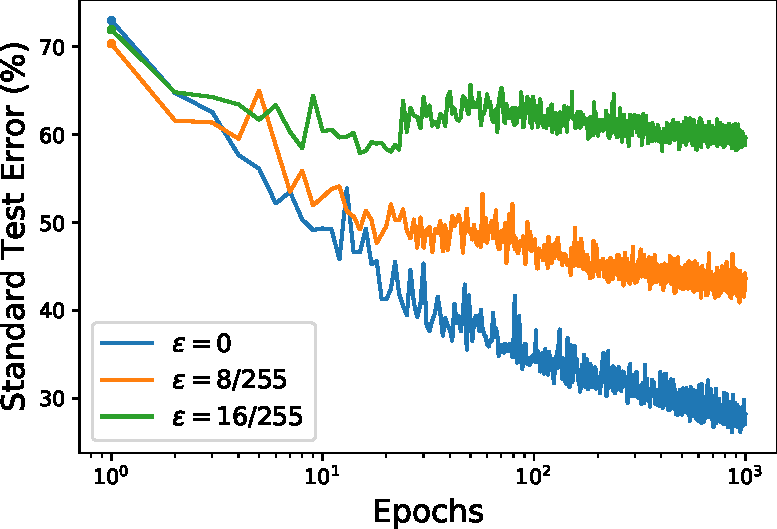
\includegraphics[width=1.0\linewidth]{figures/ad_augment.pdf}
      \caption{Standard training on a fixed adversarially augmented training set (e.g. $\varepsilon = 16/255$) can also produce prominent overfitting. In contrast, on the original training set without adversarial perturbation applied ($\varepsilon=0$), no overfitting is observed. 
      % if conducted on a dataset augmented by fixed and small adversarial perturbation, which can be properly explained by our implicit label noise perspective. 
      % Detailed experiment settings can be found in Appendix~\ref{sect: exp-ad-augment}.
      }
    \label{fig:fixed-augment}
    \vspace{-2mm}
    \end{minipage}\hfill
    \begin{minipage}{0.45\textwidth}
      \centering
      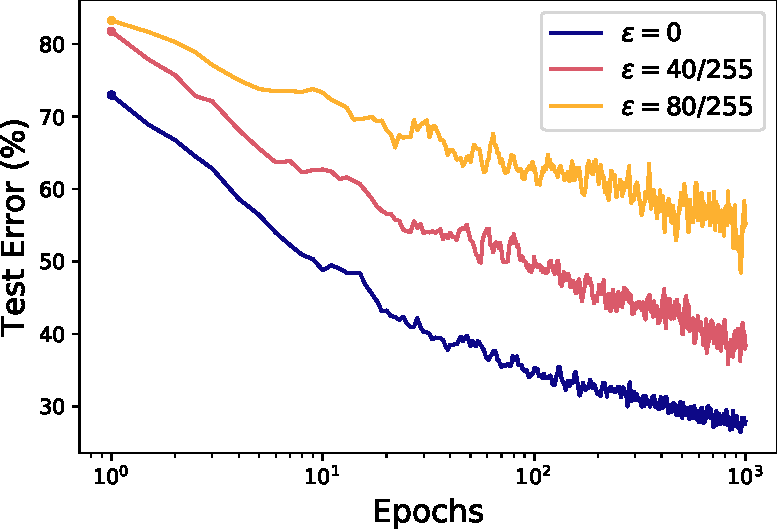
\includegraphics[width=1.0\textwidth]{figures/double-descent-gaussian-noise.pdf}
      \caption{
      Standard training on a training set augmented by Gaussian noise will not produce overfitting. Here we select extremely large perturbation radius (e.g. $\varepsilon = 80/255$) to reduce the test error to be comparable to the adversarially augmented case. 
      % Even with extremely high Gaussian noise corrupting the training set, no significant double descent can be observed. 
      }
    \label{fig:double-descent-gaussian}
    \end{minipage}
\end{figure}


% \begin{figure*}[!ht]
% \centering
% \begin{subfigure}[t]{.48\textwidth}
%   \centering
%   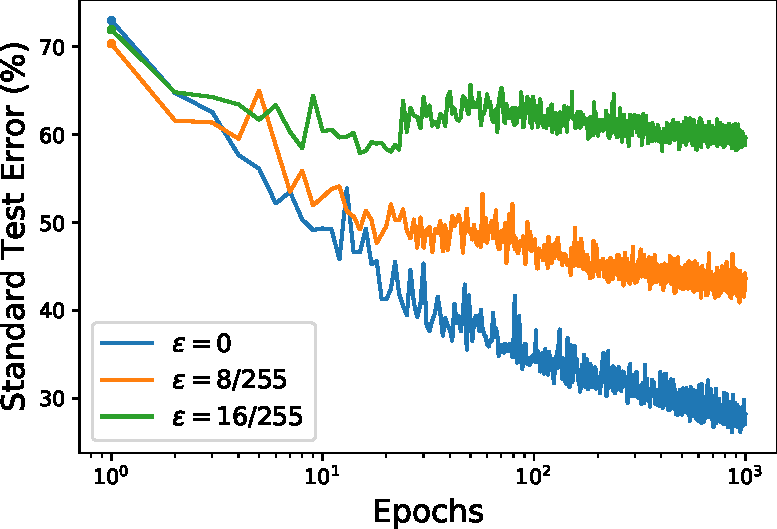
\includegraphics[width=1.0\linewidth]{figures/ad_augment.pdf}
%   \caption{Standard training on a fixed adversarially augmented training set (e.g. $\varepsilon = 16/255$) can also produce prominent overfitting. In contrast, on the original training set without adversarial perturbation applied ($\varepsilon=0$), no overfitting is observed. 
%   % if conducted on a dataset augmented by fixed and small adversarial perturbation, which can be properly explained by our implicit label noise perspective. 
%   % Detailed experiment settings can be found in Appendix~\ref{sect: exp-ad-augment}.
%   }
% \label{fig:fixed-augment}
% \vspace{-2mm}
% \end{subfigure}\hfill
% \begin{subfigure}[t]{.48\textwidth}
%   \centering
%   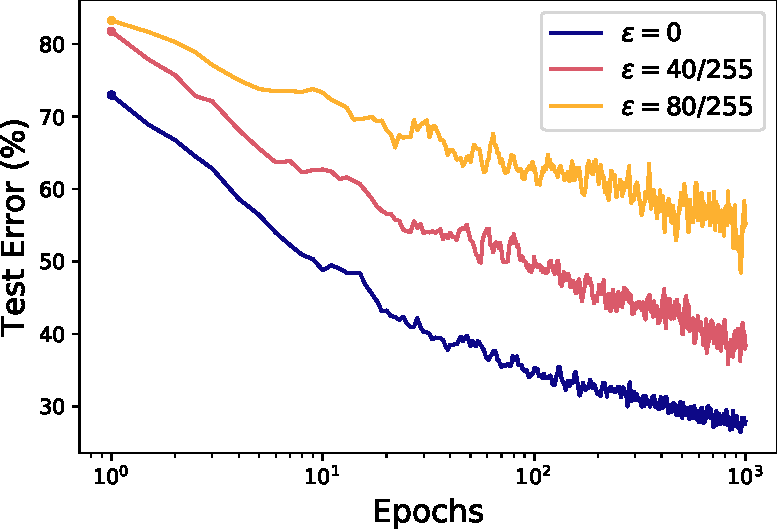
\includegraphics[width=1.0\textwidth]{figures/double-descent-gaussian-noise.pdf}
%   \caption{
%   Standard training on a training set augmented by Gaussian noise will not produce overfitting. Here we select extremely large perturbation radius (e.g. $\varepsilon = 80/255$) to reduce the test error to be comparable to the adversarially augmented case. 
%   % Even with extremely high Gaussian noise corrupting the training set, no significant double descent can be observed. 
%   }
% \label{fig:double-descent-gaussian}
% \end{subfigure}
%   \caption{}
%  \label{fig:reconcile-model}
% \end{figure*}


% \begin{figure}
% % \vspace{-2mm}
% % \vspace{-4mm}
%   \centering
%   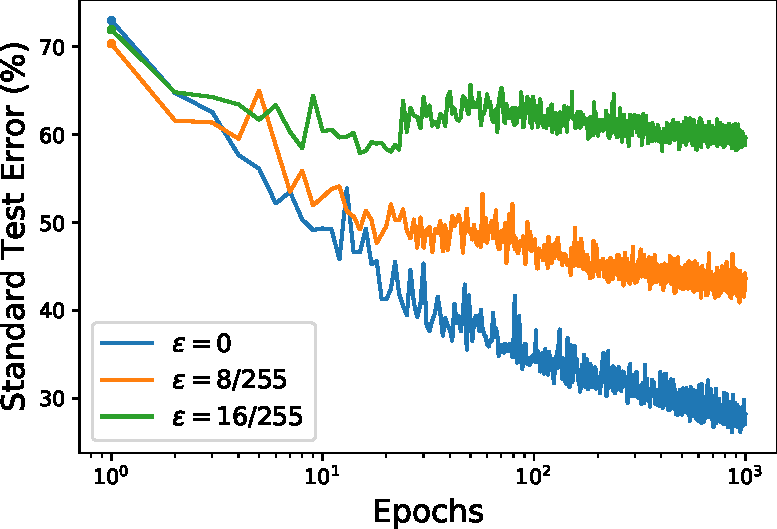
\includegraphics[width=0.5\linewidth]{figures/ad_augment.pdf}
%   \caption{Standard training on a fixed adversarially augmented training set (e.g. $\varepsilon = 16/255$) can also produce prominent overfitting. In contrast, on the original training set without adversarial perturbation applied ($\varepsilon=0$), no overfitting is observed. 
%   % if conducted on a dataset augmented by fixed and small adversarial perturbation, which can be properly explained by our implicit label noise perspective. 
%   % Detailed experiment settings can be found in Appendix~\ref{sect: exp-ad-augment}.
%   }
% \label{fig:fixed-augment}
% \vspace{-2mm}
% \end{figure}

% \begin{figure*}[!ht]
%   \centering
%   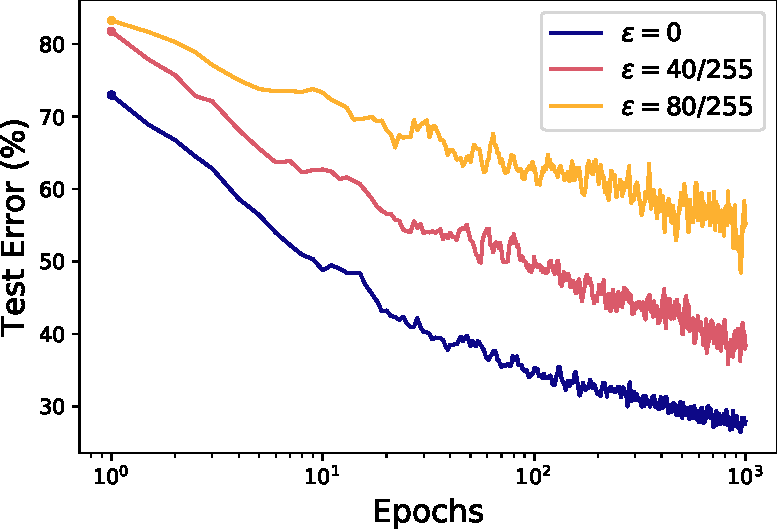
\includegraphics[width=0.5\textwidth]{figures/double-descent-gaussian-noise.pdf}
%   \caption{Even with extremely high Gaussian noise corrupting the training set, no significant double descent can be observed. This shows the input perturbation is not essential to produce double descent.
%   }
% \label{fig:double-descent-gaussian}
% \end{figure*}
    
    % Necessary conditions are that the model has to be both accurate and robust. If a model is not robust, adversarial perturbation generated by it will not induce implicit label noise. We showcase this by performing the static adversarial perturbation, namely ...
    % \todo{Adversarial perturbation generated by non-robust models will not cause double descent}, while that generated by robust models will. 
    
    
    
    
%   %%%
%     We are now ready to show that label noise implicitly exists in the adversarially augmented training set.
%     % Now we show the traditional adversarial label is improper in terms of the label distribution. 
%     As also illustrated in Figure~\ref{fig:illustration}, we have $P(\tilde{Y}' | x') = P(\tilde{Y}|x)$ by Remark~\ref{remark:common-practice} and $P(\tilde{Y}|x) = P(Y|x)$ by property of the clean dataset~(Assumption~\ref{assumption:clean-dataset}), which together means $P(\tilde{Y}' | x') = P(Y|x)$.
    
    % However, Theorem~\ref{theorem:distribution-mismatch-true-model} shows that $P(Y' | x') \ne P(Y | x)$, which implies that $P(\tilde{Y}' | x') \ne P(Y' | x')$. This means there is a mismatch between the true label distribution and the assigned label distribution of the adversarial example. 
    % Such distribution mismatch will create label noise implicitly in the adversarially augmented training set $\mathcal{D}'$.





